\section{Синтез неадаптивного и адаптивного управления, обеспечивающего	параметрическую инвариантность выхода СНС относительно неопределенности НОУ}

\begin{enumerate}
	\item Составление НОУ и эталонной модели (ЭМ)
	\item Синтез неадаптивного управления
	\item Синтез адаптивного управления
	\item Моделирование	
\end{enumerate}

\subsection{Составление НОУ и эталонной модели (ЭМ)}

Итак, для некоторого упрощения, представим ПФ НОУ~\ref{eq_OU} cо следующими обозначениями:
\begin{equation}
	\Phi(s) = \cfrac{b_1 s + b_0}{s^2 + a_1 s + a_0}
\end{equation}

И представим этот НОУ в каноническом наблюдаемом базисе векторно-матричного представления, матрицы которого равны (при величине параметрической неопределенности $[q_j] = [-0.2, 0.2]$):
\begin{align}
	A &= 
	\small
	\begin{bmatrix}
		0 & 1\\
		-a_0 & -a_1
	\end{bmatrix}
	=
	\begin{bmatrix}
		   0&          1\\      
		-0.6736 & -2.6495
	\end{bmatrix}
	+
	\begin{bmatrix}
		0 & 0\\
		[-0.4513, 0.4513]& [-1.7754, 1.7754]
	\end{bmatrix};\\
	\normalsize
	B &=
	\begin{bmatrix}
		b_1\\
		b_0
	\end{bmatrix}
	=
	\begin{bmatrix}
		0.3038\\
		0.0405
	\end{bmatrix}
	+
	\begin{bmatrix}
		[-0.0219, 0.0219]\\
		[-0.1649, 0.1649]
	\end{bmatrix};\\
	C &= 
	\begin{bmatrix}
	0 & 1
	\end{bmatrix}.
\end{align}

НОУ:
\begin{equation}
	\begin{cases}
	\dot x = A x + B u;\\
	y = C x
	\end{cases}
\end{equation}



Составим эталонную модель, коэффициенты которой зададим методом стандартных характеристических полиномов на основании заданных показателей качества замкнутой системы:
\begin{align}
	\omega_0 = 3; t_{\text{п}} = 4.8\text{ сек.}; \sigma =  0\%
\end{align}

Биноминальное разложение для ОУ второго порядка имеет вид:
\begin{equation}
	D(s) = s^2 + 2 \omega_0 s + \omega_0^2
\end{equation}

Получаем коэффициенты характеристического полинома эталонной модели:
\begin{align}
	a_{M,0} &= \omega_0^2;\\
	a_{M,1} &= 2 \omega_0.
\end{align}

Составляем матрицы эталонной модели:
\begin{align}
	A_{M} = 
	\begin{bmatrix}
		0 & 1\\
		-a_{M,0} & -a_{M,1}
	\end{bmatrix};
	B_{M} =
	\begin{bmatrix}
		0\\
		b_{M,0}
	\end{bmatrix}
\end{align}

И получаем эталонную модель:
\begin{equation}
	\begin{cases}
		\dot x_{M} = A_{M} x_{M} + B_{M} g;\\
		y_{M} = C x_{M}
	\end{cases}
\end{equation}


\subsection{Синтез неадаптивного управления}

Построим сначала неадаптивное управление в предположении, что параметры объекта точно известны. Для этого выведем модель ошибки слежения по состоянию:
\begin{equation}\label{error}
	e = x - x_{M}
\end{equation}

Дифференцируя по времени~\ref{error} с учетом НОУ и ЭМ, имеем 
\begin{equation}
	\dot e = Ax - A_{M} x_{M} + B u - B_{M} g
\end{equation}

Учтем, что
\begin{align}
	Ax - A_{M} x_{M} &= Ax - A_{M} x_{M} + A_{M} x - A_{M} x =\\&= A_{M} (x - x_{M}) + (A-A_{M}) x = A_{M} e + h \Delta^T x
\end{align}

\begin{align}
	B u - B_{M} g =
	\begin{bmatrix}
		b_1\\
		b_0
	\end{bmatrix}
	u + 
	\begin{bmatrix}
		0\\
		b_{M,0}
	\end{bmatrix}
	g
\end{align}
где 
\begin{equation}
A - A_{M} = h \Delta^T = 
\begin{bmatrix}
0\\
1
\end{bmatrix}
\begin{bmatrix}
a_0 - a_{M,0} & a_1 - a_{M,1}
\end{bmatrix}
\end{equation}

Вектор ошибок:
\begin{align}
	&\dot e_1 = e_2 + b_1 u;\\
	&\dot e_2 = -a_{M,0} e_1 - a_{M,1} e_2 + \Delta^T x + b_0 u - b_{M, 0} g 
\end{align}

Вводя обозначения:
\begin{align}
	\omega^T = 
	\begin{bmatrix}
		x^T & g
	\end{bmatrix};
	q^T = 
	\begin{bmatrix}
	\cfrac{1}{b_0} \Delta^T & -\cfrac{b_{M,0}}{b_0}
	\end{bmatrix}
\end{align}
окончательно получаем:
\begin{align}\label{typ_error}
	&\dot e_1 = e_2 + b_1 u;\\
	&\dot e_2 = -a_{M,0} e_1 - a_{M,1} e_2 + b_0 (u + \omega^T q)
\end{align}

Если выбрать в качестве ЗУ:
\begin{equation}\label{cl}
	u = - \omega^T q = - {q}_1 x_1  - {q}_2 x_2 +  {q}_3 g
\end{equation}
то, при подстановке в модель ошибок, получим 
\begin{align}
	&\dot e_1 = e_2 - b_1 \omega^T q;\\
	&\dot e_2 = -a_{M,0} e_1 - a_{M,1} e_2
\end{align}


\subsection{Синтез адаптивного управления}

Однако управление~\ref{cl} является физически нереализуемым, так как вектор параметров $q$ неизвестен. Поэтому заменим в регуляторе вектор неизвестных постоянных параметров $q$ вектором настраиваемых параметров $\hat{q}$. Получим выражение для настраиваемого регулятора вида
\begin{equation}\label{typ_cl}
	u = - \hat{q}_1 x_1  - \hat{q}_2 x_2 +  \hat{q}_3 g
\end{equation}

Подставляя~\ref{typ_cl} в~\ref{typ_error} выводим модель ошибки слежения для адаптивной системы:
\begin{align}\label{error_status}
	&\dot e_1 = e_2 + b_1 (- \hat{q}_1 x_1  - \hat{q}_2 x_2 +  \hat{q}_3 g);\\
	&\dot e_2 = -a_{M,0} e_1 - a_{M,1} e_2 + b_0 \omega^T \tilde{q}
\end{align}
где 
\begin{align}
	\tilde{q} = q - \hat{q} =
	\begin{bmatrix}
		\left(\cfrac{1}{b_0} \Delta -
		\begin{bmatrix}
		\hat{q}_1\\
		\hat{q}_2
		\end{bmatrix}
		\right)\\
		-\cfrac{b_{M,0}}{b_0} - \hat{q}_3
	\end{bmatrix}
	=
	\begin{bmatrix}
		\cfrac{a_{M,0} - a_0}{b_0} - \hat{q}_1\\
		\cfrac{a_{M,1} - a_0}{b_1} - \hat{q}_2\\
		-\cfrac{b_{M,0}}{b_0} - \hat{q}_3
	\end{bmatrix}
\end{align}

Модель~\ref{error_status} является типовой динамической моделью ошибки с измеряемым состоянием. С учетом принятых в этот разделе обозначений  алгоритм адаптации принимает вид:
\begin{equation}
	\dot{\hat{q}} = \gamma \omega h^T P e
\end{equation}
где $\gamma > 0$~-- коэффициент адаптации,
\begin{align}
	h^T P e = p_{2,1} e_1 + p_{2,2} e_2,
\end{align}
а симметрическая положительно определенная матрица $P$ является решением уравнения:
\begin{equation}\label{sylv_err}
	A_{M}^T P + P A_{M} = -Q, Q = Q^T > 0
\end{equation}

Для расчета матрицы $P$ зададимся симметрической положительно определенной матрицей $Q$:
\begin{equation}
	Q = 
	\begin{bmatrix}
		100 & 0\\
		0 & 10
	\end{bmatrix}
\end{equation}

Тогда при решении уравнения~\ref{sylv_err} получим реализацию матрицы $P$:
\begin{equation}
	P = 
	\begin{bmatrix}
		p_{11} & p_{12}\\
		p_{21} & p_{22}
	\end{bmatrix}
	=
	\begin{bmatrix}
	  -49.16 & -5.56\\
	-5.56 & -1.76	
	\end{bmatrix}
\end{equation}

\subsection{Моделирование}

Результаты моделирования приведены для $\omega_0 = 10, \gamma = 30$.

\begin{figure}[h!]
	\centering
	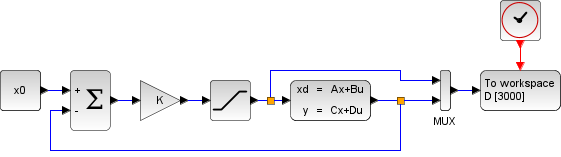
\includegraphics[width=1\textwidth]{model.png}
	\caption{Схема моделирования -- ОУ и Регулятор}
	\label{}
\end{figure}

\begin{figure}[h!]
	\centering
	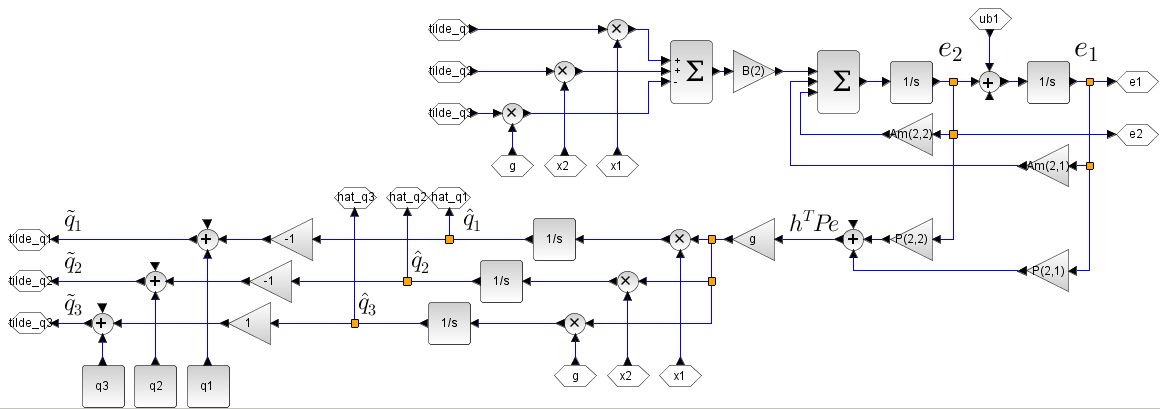
\includegraphics[width=1\textwidth]{error_model.png}
	\caption{Схема моделирования -- Модель ошибки}
	\label{}
\end{figure}
\newpage
\begin{figure}[h!]
	\centering
	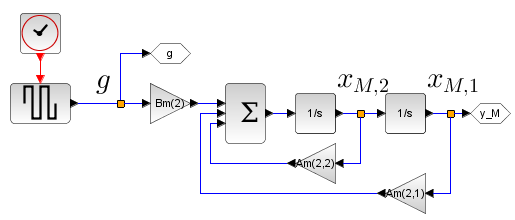
\includegraphics[width=0.8\textwidth]{sm.png}
	\caption{Схема моделирования -- Эталонная модель}
	\label{}
\end{figure}

\begin{figure}[h!]
	\centering
	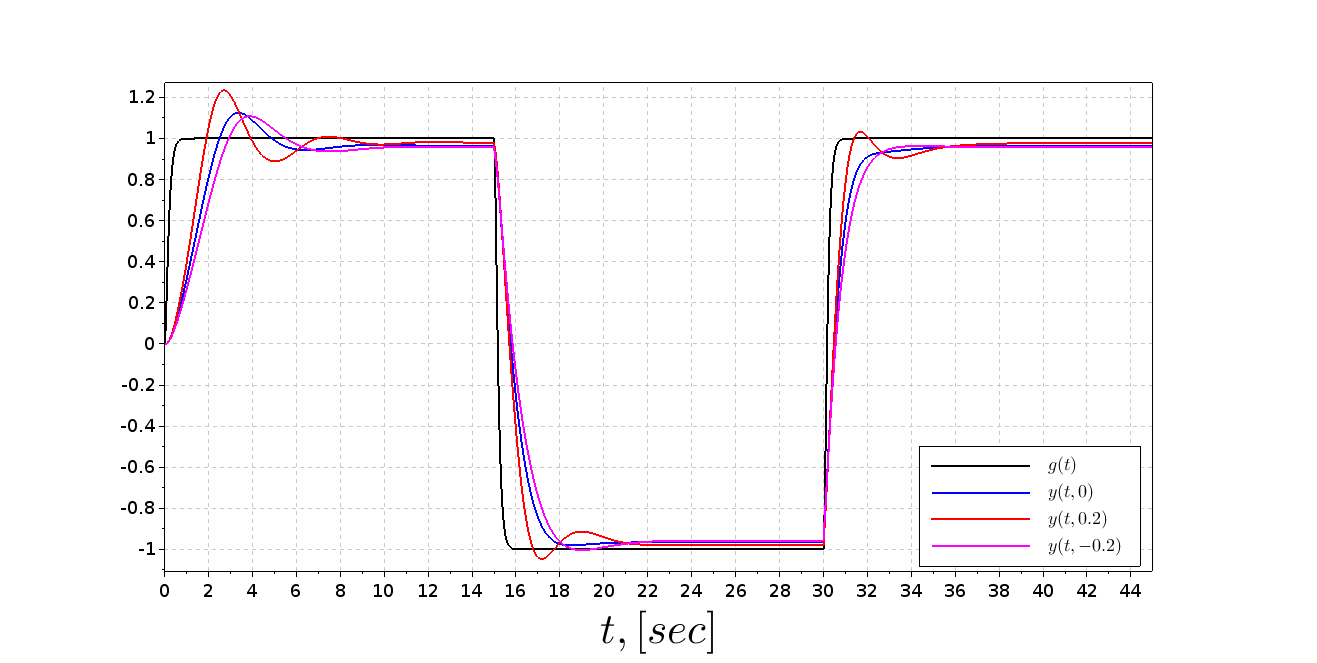
\includegraphics[width=1\textwidth]{adaptiv_square_y.png}
	\caption{Результаты моделирования -- Выходной сигнал при вариации вектора $q_j$}
	\label{}
\end{figure}
\newpage
\begin{figure}[h!]
	\centering
	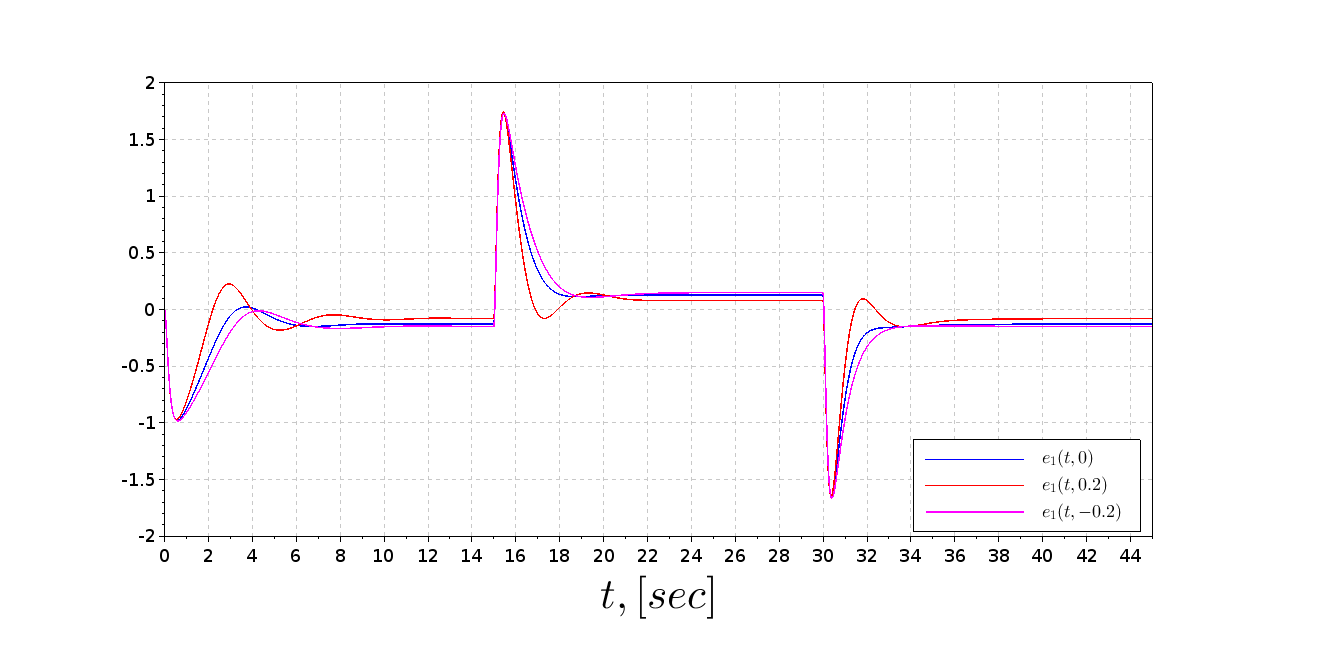
\includegraphics[width=1\textwidth]{adaptiv_square_error.png}
	\caption{Результаты моделирования -- Выходной сигнал модели ошибки $e_1$ при вариации вектора $q_j$}
	\label{}
\end{figure}



\newpage 